\section{Hypothesis Testing}

We focused a lot to derive good surrogate losses for the 0-1 loss. But is this error really a good metric? Hypothesis testing is a way to express asymmetry in classification tasks. For this we introduce the confusion matrix:

\begin{center}
	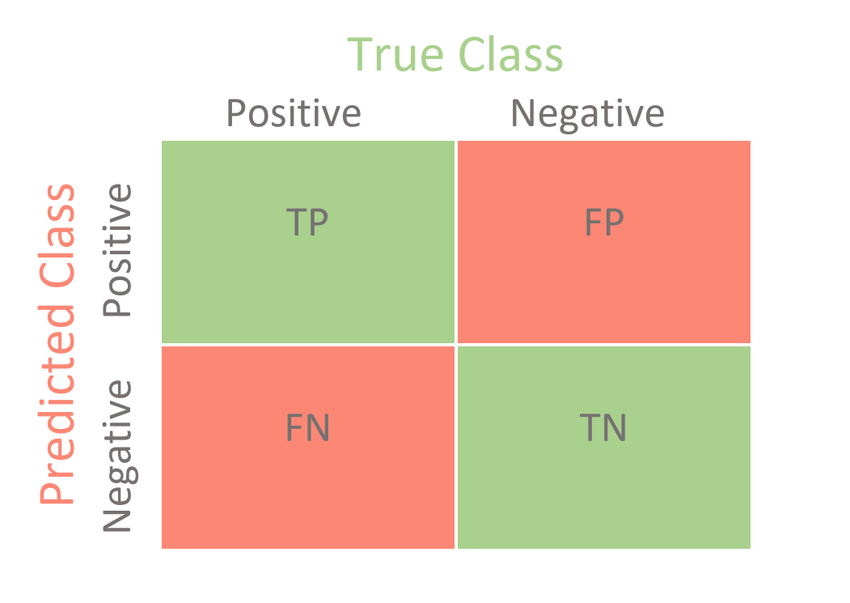
\includegraphics[width=0.85\columnwidth]{confusion-matrix.png}
\end{center}

Further we define:
$$\text{error}_1 / \text{FPR} = \frac{FP}{TN + FP}, \quad \text{error}_2 / \text{FNR} = \frac{FN}{TP + FN}$$

We want to find a test that minimizes the FPR, while controlling the FNR. This can be viewed as defining a null hypothesis $H_0(x)$ and then deciding to accept or reject it ($H_0$ is always the positive class). When choosing $H_0$ we want it to represent the more crucial class one to get right, e.g. it is more important to truly classify a person as sick than to classify them as healthy. To decide it we accept or reject $H_0$ we fix $\tau$, where we accept $H_0(x) (\hat{y} = -1)$ if $\hat{p}(x) < \tau$ and the opposite way around.

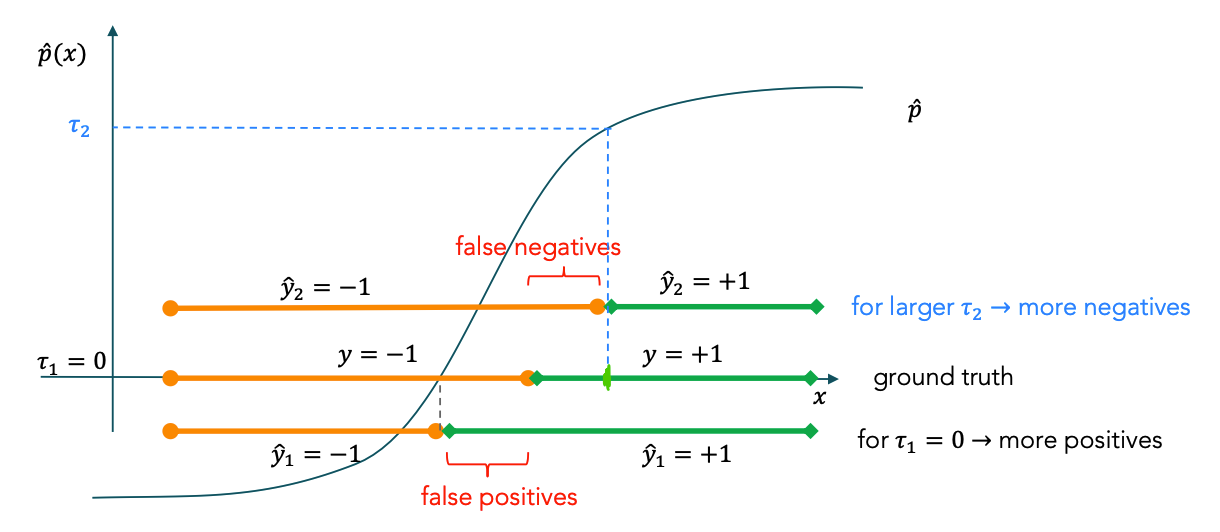
\includegraphics[width=\columnwidth]{fp-fn-tradeoff.png}

\subsection{AUROC}

We want to have a large recall $\frac{TP}{\#[y = +1]}$ but also a small FPR. Based on these metrics we can draw the ROC curve by varying $\tau$.

\begin{center}
	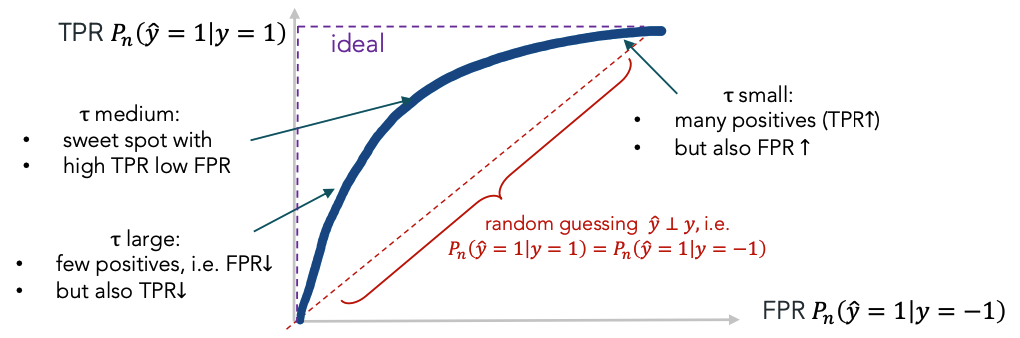
\includegraphics[width=0.87\columnwidth]{roc.png}
\end{center}

We can either choose our model by caring about a specific point, e.g. TPR $@$ FPR = 5\%, or we choose whichever courve gets closer to the ideal curve, that is maximizing the area under the curve.